\subsection{Программная реализация устройства стратегического управления}
Устройством стратегического управления является одноплатный миникомпьютер «Rasp- berry Pi Zero W 2» (Рисунок 3.3), система запускается сразу после подачи питания на устройство. Происходит запуск операционной системы «Linux» и ожидание подключения пользователя к устройству. Возможен два варианта использования стратегического устройства:

\begin{enumerate}
	\item Подключение по беспроводному каналу, по протоколу SSH.
	\item Через проводное подключение, путем подключения проводов монитора и устройств ввода/вывода.
\end{enumerate}

Для подключения мини-компьютера по беспроводному каналу, необходимо чтобы микрокомпьютер был в локальном окружении беспроводной сети.

Для дальнейшей работы управления используется один из языков высокого уровня, например, язык программирования Python c использованием библиотек, пример представлен на рисунке \ref{CodePython1}.
\begin{figure}[H]
	\centering

	\begin{minted}[tabsize=2,breaklines,fontsize=\small]{python}
import numpy as np
from pybotics.geometry import vector_2_matrix
poses = np.array([
    vector_2_matrix([600, -150, 800,
                     np.deg2rad(-90), 0,
                     np.deg2rad(-90)]),
    vector_2_matrix([700, -150, 800,
                     np.deg2rad(-90), 0,
                     np.deg2rad(-90)])
])
start_end_joints = [robot.ik(p) for p in poses]
	\end{minted}
	\caption{Фрагмент использования сторонних библиотек на языке питон.}\label{CodePython1}
\end{figure}


При помощи библиотек возможно производить программирование робота в режиме симуляции и только потом генерировать команды для контроллера тактического управления. Использования языка высокого уровня позволяет создавать комплексные стратегии движения и обрабатывать сложные алгоритмы. Для коммуникации между устройствами стратегического и тактического уровня предполагается использование написанного библиотеки API, пример функции представлен на Рис. \ref{CodePython2} для общения между микроконтроллером и микрокомпьютера


\begin{figure}[H]
	\centering

	\begin{minted}[tabsize=2,breaklines,fontsize=\small]{python}
def send_movej_command(self, command):
    """
    Send a moveJ command to the robot through the serial connection.
    Args:       
    serial_connection (serial.Serial): The serial connection to the robot.
    command (str): The moveJ command string.
    """
    with serial.Serial(self.serial_port, self.baud_rate, timeout=1) as ser:
  	log("Serial connection established.")
    serial_connection.write(command.encode())
    	log(f"Sent command: {command}")
    if self.ser.in_waiting:
	response = self.ser.read(ser.in_waiting).decode()
          log("Received response:", response)
	\end{minted}
	\caption{Фрагмент функции API библиотеки для использования на языке Python.}\label{CodePython2}
\end{figure}


Так же ещё одним возможным видом программирования является использование программного обеспечение RoboDK, на устройстве стратегического управления исполняется драйвер, который передает данные из сокетного TCP/IP соединения в Uart, список команд рассматривается в таблице 5.1 на контроллер тактического управления фрагмент представлен в приложение 2.

\begin{table}[H]
	\caption{Список базовых команд который поддерживает robotDK}\label{TRobotDK}
	\begin{adjustbox}{width=\textwidth}

		\begin{tabular}{|l|l|l|l|}
			\hline
			Command    & Description                                             & Parameters                                     & Example 			Usage             \\ \hline
			MOVJ       & Moves 			the robot joints to specified positions.       & Joint 			Positions (degrees or radians)        & MOVJ 			10 20 30 40 50 60 70 \\ \hline
			CJNT       & Requests 			the current joint positions.                & None                                           & CJNT                         \\ \hline
			MOVL       & Moves 			the robot to a specified linear position.      & Cartesian 			Coordinates (X, Y, Z, Rx, Ry, Rz) & MOVL 			500 400 300 0 1.57 0 \\ \hline
			SPEED      & Sets 			the movement speed of the robot.                & Speed 			Value (units per minute)              & SPEED 			500                 \\ \hline
			WAIT       & Pauses 			the robot operation for a specified duration. & Time 			(seconds)                              & WAIT 			5                    \\ \hline
			STOP       & Stops 			all robot movements immediately.               & None                                           & STOP                         \\ \hline
			DISCONNECT & Terminates 			the connection with the robot.            & None                                           & DISCONNECT                   \\ \hline
		\end{tabular}
	\end{adjustbox}

\end{table}

\subsection{Алгоритмы устройства исполнительного управления}

Главная цель исполнительной системы управления плавное управление 3х фазным BLDC двигателем для этого необходимо считывать, обрабатывать данные с датчиков положения и тока и производить генерацию сигналов PWM. На рисунке \ref{ACDALG} показан основной алгоритм работы системы исполнительного устройства.


\begin{figure}[H]
	\centering
	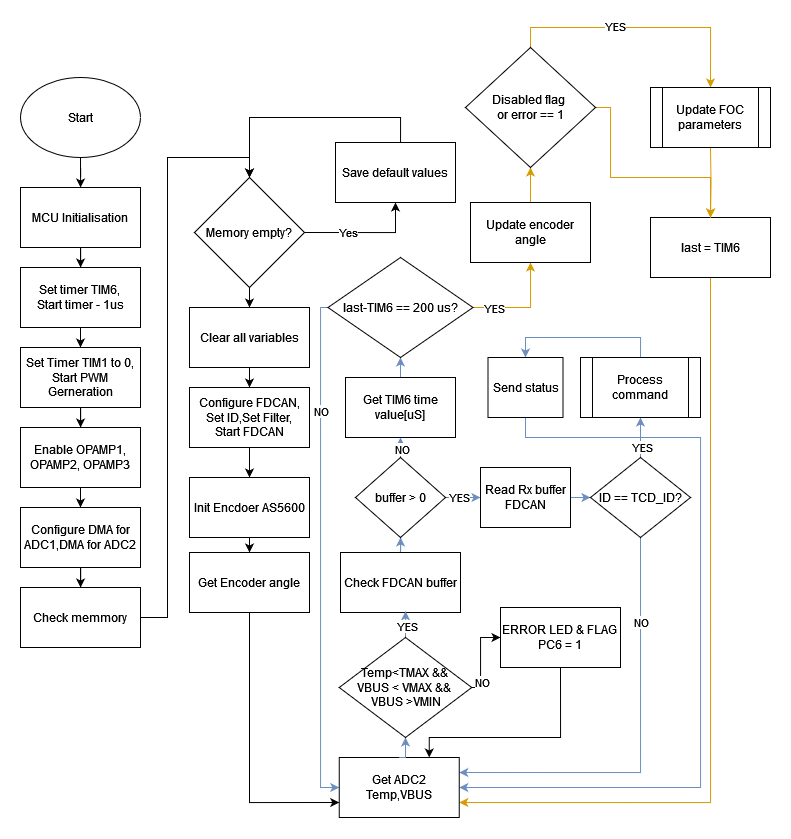
\includegraphics[width=\textwidth]{Src/images/ACD ALG.png}
	\caption{Алгоритм работы системы исполнительной системы.}
	\label{ACDALG}
\end{figure}

После включения микроконтроллер проводит проверку всех устройств на работоспособность путем считывания данных. Система разделена  на две части, в первой части выполняются функци, которые не требуют частого выполнения (окрашено желтым цветом), вторая выполняется на максимальной большой частоте, с которой возможно выполнение, такими задачами являются вычисление векторного алгоритма и парсинг сообщений Рисунок \ref{ACDCMDALG}.

\begin{figure}[H]
	\centering
	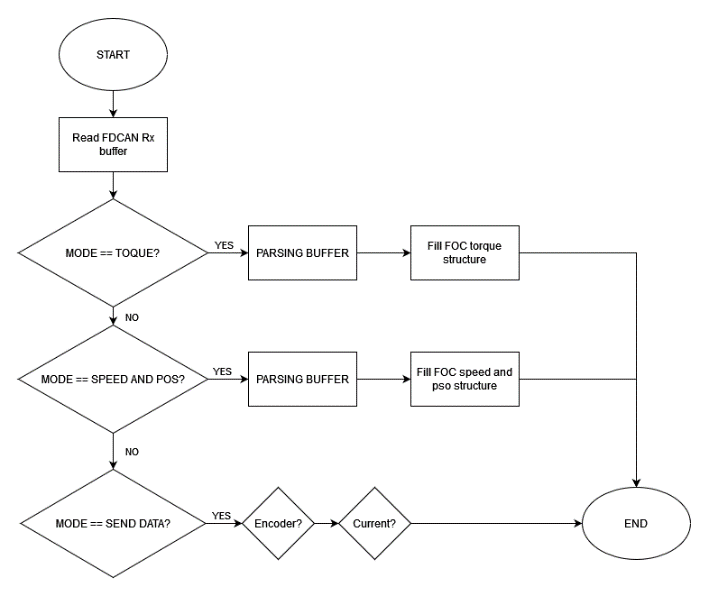
\includegraphics[width=\textwidth]{Src/images/ACDCMDALG.png}
	\caption{Алгоритм обработки сообщения.}
	\label{ACDCMDALG}
\end{figure}

Рисунок 5.8 показывает схема работы векторного регулирования. В качестве примера произведен пример управления по току с обратной связью, что означает, что двигатель всегда создает постоянный крутящий момент (то есть постоянный ток, поскольку крутящий момент пропорционален току).

Входы $i_q$ и $i_d$ регулируются с помощью обратной связи через ПИД-регулятор, который также включает в себя несколько модулей преобразования «Park» и «Clark», сигналы проходят через блок «SVPWM» \citep{Ananth2012} (Широтно-импульсная модуляция с пространственным вектором) и происходит воздействие на трехфазный инвертор для управления двигателем, а величина обратной связи ПИД-регулятора представляет собой выборочное значение выходного тока двигателя.

\begin{figure}[H]
	\centering
	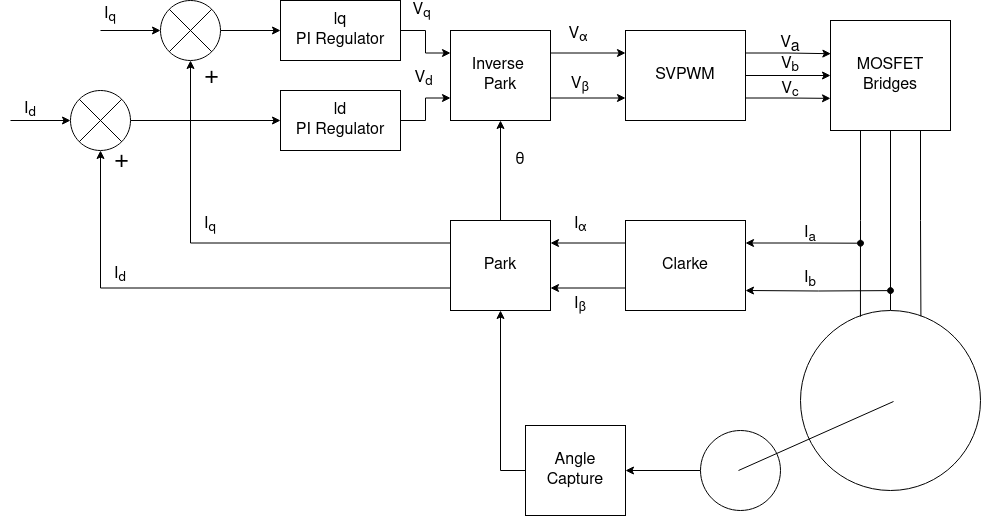
\includegraphics[width=\textwidth]{Src/images/FOC maindrawio.png}
	\caption{Схема векторного управления двигателем.}
	\label{ACDFOCALG}
\end{figure}


Весь процесс векторного управления можно разбить на этапы:
\begin{enumerate}
	\item Получение данных трехфазного тока двигателя для вычисления значений $I_a,I_b$;
	\item Преобразование $I_a,I_b,I_c$ методом Clark, получение $I_\alpha,I_\beta$;
	\item Преобразование $I_\alpha,I_\beta$ методом Park, получение $I_q,I_d$;
	\item Вычисление ошибки $I_q,I_d$; из значений установки $I_q,I_d$ поступающих от контроллера;
	\item Ведение указанной ошибки в два ПИД-регулятора (используется только ПИ), для получения выходных управляющих напряжений $V_q,V_d$;
	\item Преобразование $V_q,V_d$ методом обратным превращением Park, получение $V_\alpha,V_\beta$;
	\item Использование пространственного вектора $V_\alpha,V_\beta$ для определения сигналов широтно-импульсной модуляции для трех полумостов инвертора;
	\item Управление силовыми MOSFET транзисторами трехфазного инвертора в соответствии с ранее выведенным кодовым значением для привода двигателя;
	\item Повторение вышеуказанных шагов;
\end{enumerate}

В вычислениях достаточно использовать только ток с двух фаз мотора, так как по закону тока Кирхгофа можно рассчитать третью составляющую тока, ведь сумма токов, втекающих в узел, равна сумме токов, вытекающих из узла $I_a+I_b+I_c=0$. Вектора $I_a,I_b,I_c$ изначально не ортогональны, для дальнейшей работы требуется провести перерасчет проекции в оси координат, формула \ref{Clark}.
\begin{ceqn}
	\begin{align} \label{Clark}
		\begin{cases}
			I_{\alpha} = I_a - \cos\left(\frac{2\pi}{3}\right) I_b - \cos\left(\frac{2\pi}{3}\right) I_c \\
			I_{\beta} = \sin\left(\frac{2\pi}{3}\right) I_b - \sin\left(\frac{2\pi}{3}\right) I_c
		\end{cases}
	\end{align}
\end{ceqn}

После преобразования получается синусоидальная волна, но на одну переменную меньше. Теперь можно использовать значения $I_\alpha,I_\beta$ для управления вращением двигателя, заставляя их соответствовать правилам изменения формы сигнала. Для применения к трем фазам двигателя применяется обратное преобразование Кларка.
Преобразование Park, формула \ref{Park}, главная задача перевести стационарную систему $I_\alpha,I_\beta$ в cистему координат вращающейся вместе с ротором $I_q,I_d$, а так как в системе подразумевается получать данные положения угла поворота двигателя с энкодера в реальном времени. Получается, что вектор вращения становится фиксированным значением в системе координат$I_\alpha,I_\beta$.  Далее использование $I_q,I_d$ в качестве объектов управления как обратную связь через ПИД-регулятор. В реальности используется только ПИ-регулятор, дифференциальный регулятор не вводится, потому как передаточная функция напряжения и тока является инерционным звено первого порядка.

\begin{ceqn}
	\begin{align} \label{Park}
		\begin{cases}
			I_d = I_\alpha \cos(\theta) + I_\beta \sin(\theta) \\
			I_q = -I_\alpha \sin(\theta) + I_\beta \cos(\theta)
		\end{cases}
	\end{align}
\end{ceqn}




\begin{figure}[H]
	\centering
	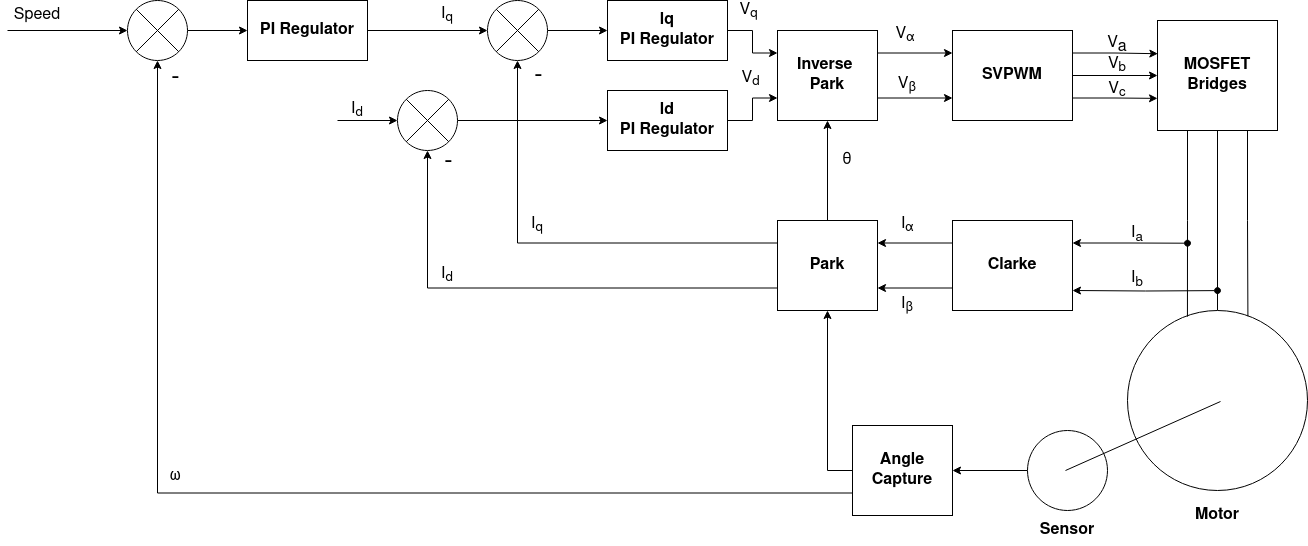
\includegraphics[width=\textwidth]{Src/images/speed.drawio.png}
	\caption{Схема векторного управления двигателем по скорости.}
	\label{ACDFOCALGSPD}
\end{figure}

В обычном векторным управлении в основном используются три контура ПИД: контур тока, контур скорости и контур положения, то есть: управление током двигателя (крутящим моментом) посредством обратной связи по току -> затем управление скоростью двигателя, контролируя крутящий момент -> затем управление положением двигателя, контролируя скорость двигателя.

На картинке выше \ref{ACDFOCALGSPD}, $\omega$  — это обратная связь по скорости двигателя, которую рассчитывается с помощью энкодера двигателя. Она контролируется PI регулятором.

Расчетная скорость двигателя и значение настройки скорости вычисляет значение ошибки и подставляет его в контур ПИ скорости. Вычисленный результат используется в качестве входного сигнала токового контура, таким образом реализуя двойное регулирование скорости-тока с обратной связью.

Самый внешний уровень — это контур положения, который управляет двигателем, поворачивая его на точный угол и поддерживая его. Блок-схема управления изображено на картинке \ref{ACDFOCALGPOS}.

\begin{figure}[H]
	\centering
	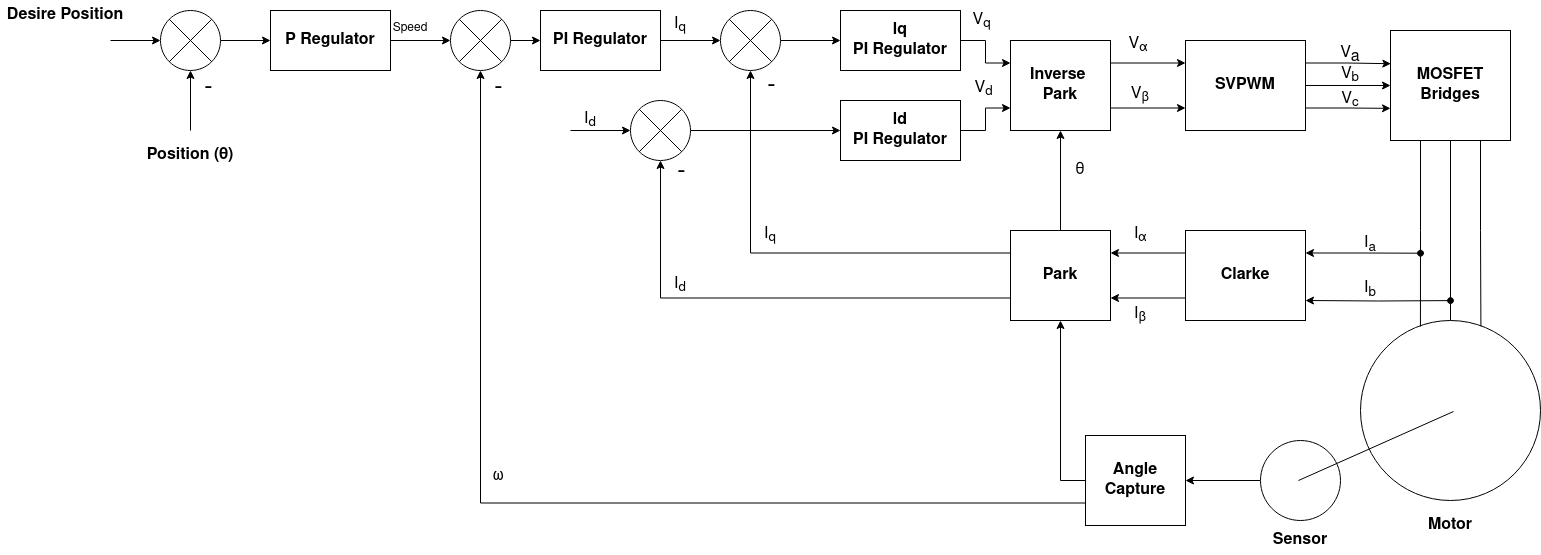
\includegraphics[width=\textwidth]{Src/images/Foc pos.drawio.png}
	\caption{Схема векторного управления двигателем по положению.}
	\label{ACDFOCALGPOS}
\end{figure}


Но в реальном использовании алгоритма применительно к системе, энкодер не может напрямую возвращать скорость двигателя. Поэтому скорость двигателя рассчитывается, вычислив изменение значения кодирования в течение определенного периода времени (то есть используя среднюю скорость для представления мгновенной скорости). Когда скорость двигателя относительно высока, этот метод подходит, но в режиме управления положением скорость двигателя будет очень низкой (поскольку ротор необходимо зафиксировать в определенном положении).
Поэтому, чтобы избежать ошибок, вызванных связью скорости, для управления положением  используется только двойной контур, состоящий из положения и тока. Однако в это время необходимо внести определенные изменения в контур положения Рисунок \ref{ACDFOCALGPOSREAL}.

\begin{figure}[H]
	\centering
	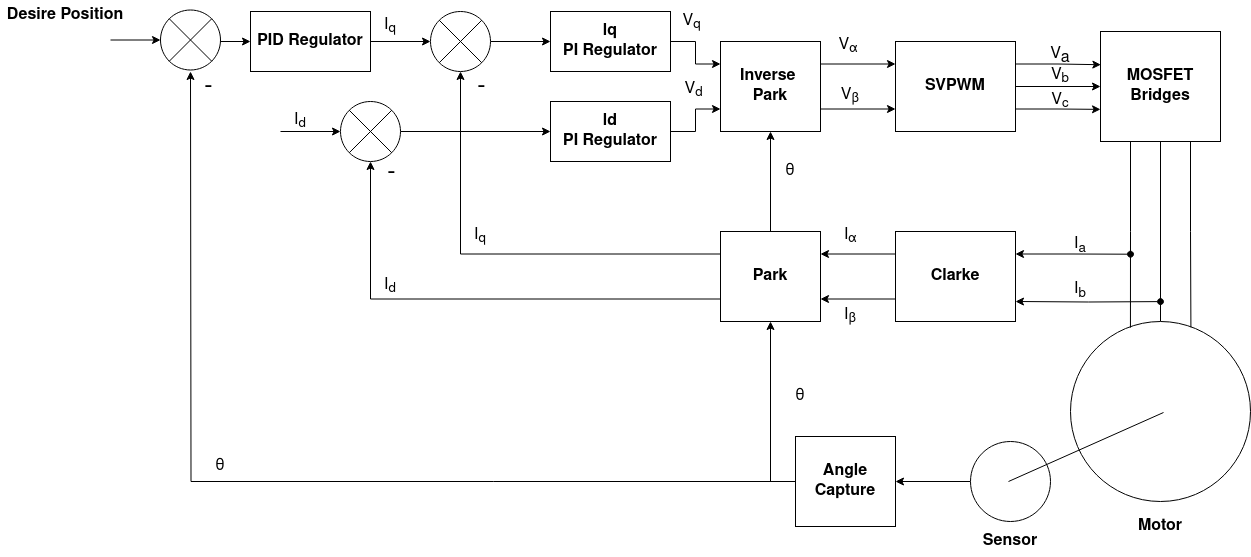
\includegraphics[width=\textwidth]{Src/images/foc pos real.drawio.png}
	\caption{Схема оптимального векторного управления двигателем по положению.}
	\label{ACDFOCALGPOSREAL}
\end{figure}

Но так же учитывается, что контур скорости удален, используется полное ПИД-управление для контура положения, то есть добавляем дифференциальный член (поскольку дифференциал положения — это скорость, это может уменьшить колебания регулирования положения и ускорить сходимость, функция интегрального члена заключается в устранении статической ошибки).



Для преобразования непосредственно в сигналы подаваемые на силовые транзисторы используется метод SVPWM (Space Vector Pulse Width Modulation), так он является наиболее эффективен, чем SPWM \citep{Mirdas2023}.

\begin{figure}[H]
	\centering
	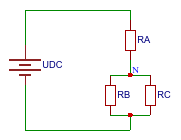
\includegraphics[width=0.3\textwidth]{Src/images/3phasesimpl.png}
	\caption{Эквивалентная схема.}
	\label{ACDFOC3P}
\end{figure}

Для понимая процесса формирования сигналов необходимо понимание вектора космического напряжения. Можно представить подключение двигателя к источнику напряжения как Рис.\ref{ACDFOC3P}.

Трехфазные напряжения (фазное напряжение — это напряжение каждой фазы относительно средней точки подключения двигателя)  выражается по формуле \ref{3ph}:
\begin{ceqn}
	\begin{align} \label{3ph}
		\begin{cases}
			U_a & = U_A - U_N = \frac{2}{3} U_{dc}  \\
			U_b & = U_B - U_N = -\frac{1}{3} U_{dc} \\
			U_c & = U_C - U_N = -\frac{1}{3} U_{dc}
		\end{cases}
	\end{align}
\end{ceqn}
Можно представить, что три напряжения формируют векторы $\vec{U_a}, \vec{U_b}, \vec{U_c}$, которые формируют результирующий вектор $\vec{U}$, получается возможно определить вектор магнитного поля. А так как постоянный магнит ротора будет стремиться вращаться до тех пор, пока линии внутреннего магнитного поля не будут соответствовать направлению внешнего магнитного поля, этот вектор может фактически представлять направление, в котором мы хотим, чтобы ротор вращался. Получается возможно рассчитать вектор пространственного напряжения \ref{spwm} \citep{youtuFieldOriented}.


\begin{ceqn}
	\begin{align} \label{spwm}
		\begin{cases}
			U_A(t) = U_{dc}\cos(2\pi ft)                             \\
			U_B(t) = U_{dc}\cos\left(2\pi ft - \frac{2\pi}{3}\right) \\
			U_C(t) = U_{dc}\cos\left(2\pi ft + \frac{2\pi}{3}\right)
		\end{cases}
	\end{align}
\end{ceqn}


Метод SVPWM позволяет синтезировать значение SPWM в каждом моменте времени\ref{SVPWMF}.
\begin{ceqn}
	\begin{align} \label{SVPWMF}
		\int_0^T U_{\text{ref}} \, dt = \int_0^{T_x} U_x \, dt + \int_{T_x}^{T_x+T_y} U_y \, dt + \int_{T_x+T_y}^T U^*_0 \, dt
	\end{align}
\end{ceqn}

\begin{ceqn}
	\begin{align} \label{SVPWM}
		U_{\text{reference}} \cdot T = U_x \cdot T_x + U_y \cdot T_y + U_0^* \cdot T_0^*
	\end{align}
\end{ceqn}

Так программа в микроконтроллер использует дискретизацию, может упростить до \ref{SVPWM}, где $U_{\text{reference}}$ — ожидаемый нами вектор напряжения, а $T$ — период ШИМ. Cмысл приведенной выше формулы заключается в периодическом переключении между различными векторами пространственного напряжения, в котором можно синтезировать эквивалентный произвольный вектор пространственного напряжения.



\subsection{Программная реализация устройства исполнительного управления}

Программа для микроконтроллера разрабатывалась на языке C/C++, для облегчения и ускорении разработки использовалась библиотека HAL (Hardware Abstraction Layer). Набор библиотек позволяет прейти но мледующий уровень абстракции и позволяет производить перенос программного кода на микроконтроллеры другого семейства. Для генерации и настройки проекта использовался инструмент графической конфигурации STM32CubeMX. Генерация проекта производилось под среду интегрированной разработки STM32CubeIDE, которая является изменненой средой разрабоки Eclipse для встроенных систем. На рисунке \ref{STM32G431MX} представленно графическое отображение настройки тактирования тактовой частоты и частоты тактирования отдельных периферийных блоков. МК контроллер работает на максимальной частоте с учетом использования внешнего кварцевого резонатора на 8 Mhz, Входная частота поступает на блок фазовой автоподстройки частоты (PLL), далее происходит умножение и деление частоты до выходной частоты, которая достигает уровня 94% от максимальной, тоесть 160 Mhz.


\begin{figure}[H]
	\centering
	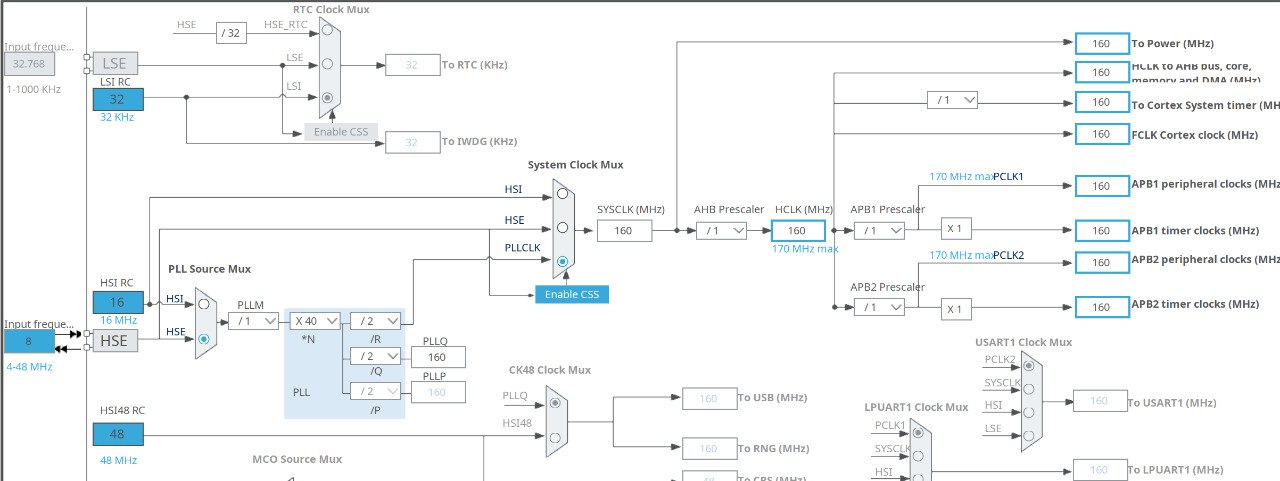
\includegraphics[width=\textwidth]{Src/images/CubeMX.png}
	\caption{Графическое отображение тактирования микроконтроллера STM32G431}
	\label{STM32G431MX}
\end{figure}


Энкодер устанавливается на роторе двигателя совместно с редуктором, необходимо было решить проблему сохранения угла поворота. Для этого был создан алгоритм сохранения угра поворота, при варианте поворота энкодера от 0 до 360 градусов. В проложении 3 реализован тест на языке Python алгоритма угла поворота энкодера.
Для обеспечения считывания данных о положении ротора микрокотроллер отправляет запрос данных у энкодера AS5600, после чего функция заполняет функция заполняет структуру данных, фрагмент фрагмент когда функции показан на картинке \ref{codeencoder}.



\begin{figure}[H]
	\centering
	\begin{minted}[tabsize=2,breaklines,fontsize=\small]{cpp}
angle_t data;
data.raw = 0;
  if(HAL_I2C_Mem_Read(a->i2cHandle,a->adress,0x0E,I2C_MEMADD_SIZE_8BIT, (uint8_t*)&data.raw,2,2)!= HAL_OK) 
{
  status = HAL_ERROR;
}
  *angle = ((data.bit.angleHIGH << 8) & 0xF00) | data.bit.angleLOW;
}
	\end{minted}
	\caption{Фрагмент кода функции считывания данных с энкодера.}\label{codeencoder}
\end{figure}


Энкодер устанавливается непосредственно на валу электродвигателя, вращение двигателя превосходят границы измеряемых параметров абсолютного энкодера AS5600 от 0 до 360 градусов (так как используется редуктор), поэтому возникла необходимость измерения угла поворота в более широком диапазоне, функция измеряет значения текущего положения, скорости и ускорения представлен в приложении 4.


%\subsection{Алгоритмы устройства тактического управления}



\subsection{Программная реализация устройства тактического управления}


В процессе различных вычислений необходимо операции, которые выходят за рамки стандартных библиотек С++. При вычислении используются часто перемножение матриц, было реализована функция перемножения двух матриц, которая показана на Рис. \ref{codematrix}. Функция для умножения матриц реализована так, что она принимает на вход три указателя на массивы, представляющие две входные матрицы и одну выходную матрицу, а также три целочисленных значения, указывающих размеры этих матриц. Входные матрицы обозначены как первая и вторая, а результат их умножения записывается в выходную матрицу.

Для выполнения умножения матриц, функция задействует три вложенных цикла, где каждый цикл отвечает за свою часть процесса: внешний цикл перебирает строки первой матрицы, средний цикл - столбцы второй матрицы, а внутренний цикл занимается элементами текущих строк и столбцов, участвующих в вычислении. Это позволяет последовательно вычислить значения для каждой ячейки результирующей матрицы.

В процессе умножения для каждой пары строки и столбца входных матриц вычисляется скалярное произведение соответствующих векторов. Для этого элементы строки первой матрицы поочерёдно умножаются на соответствующие элементы столбца второй матрицы, а результаты сложения этих произведений формируют значение в ячейке результирующей матрицы.

Таким образом, каждый элемент выходной матрицы является суммой произведений элементов соответствующих строки и столбца входных матриц, что и обеспечивает результат умножения матриц.

\begin{figure}[H]
	\centering
	\begin{minted}[tabsize=2,breaklines,fontsize=\small]{cpp}
    void MultiplyMatrices(const float* matA, const float* matB, float* resultMat, int rowsA, int commonDim, int colsB) {
    float sum;
    int rowIdx, colIdx, kIdx;
    // Loop through each row of the first matrix
    for (rowIdx = 0; rowIdx < rowsA; rowIdx++) {
        // Loop through each column of the second matrix
        for (colIdx = 0; colIdx < colsB; colIdx++) {
            sum = 0.0f; // Temporary variable to store sum
            // Multiply elements across the common dimension
            for (kIdx = 0; kIdx < commonDim; kIdx++) {
                sum += matA[commonDim * rowIdx + kIdx] * matB[colsB * kIdx + colIdx];
            }
            // Assign the computed sum to the result matrix
            resultMat[colsB * rowIdx + colIdx] = sum;
        }
    }
    }
	\end{minted}
	\caption{Функция для умножения двух матриц}\label{codematrix}
\end{figure}

Функция для преобразования матрицы поворота в углы Эйлера, рисунок \ref{codeConvertRotationMatrixToEulerAngles}, принимает два аргумента: первый аргумент — это указатель на входную матрицу поворота, второй аргумент — указатель на массив, в который будут записаны рассчитанные углы Эйлера.

В начале функции объявляются переменные для трех углов Эйлера: рыскание (yaw), тангаж (pitch) и крен (roll), а также переменная для косинуса тангажа. Эти переменные используются для хранения промежуточных вычислений и итоговых результатов преобразования.

Далее следует проверка на условие, когда матрица поворота находится в состоянии, известном как "гимбал лок". Это состояние возникает, когда одна из осей вращения становится неопределенной из-за параллельности двух других осей. Условие гимбал лока определяется значением элемента матрицы поворота, и если это значение близко к 1 или -1, выполняется специальная обработка для расчета углов Эйлера.



\begin{figure}[H]
	\centering
	\begin{minted}[tabsize=2,breaklines,fontsize=\small]{cpp}
    void ConvertRotationMatrixToEulerAngles(const float* rotationMatrix, float* angles){
        float roll, pitch, yaw, cosPitch;
        // Check for gimbal lock
        if (fabs(rotationMatrix[6]) >= 1.0 - 0.0001){
            // Handle the gimbal lock case
            roll = 0.0f;  // Set roll to zero as it's indeterminate
            if (rotationMatrix[6] < 0) {
                pitch = (float) M_PI_2;  // 90 degrees
                yaw = atan2f(rotationMatrix[1], rotationMatrix[4]);
            }
            else{
                pitch = -(float) M_PI_2;  // -90 degrees
                yaw = -atan2f(rotationMatrix[1], rotationMatrix[4]);
            }
        }else{
            // Regular case, no gimbal lock
            pitch = atan2f(-rotationMatrix[6], sqrtf(rotationMatrix[0] * rotationMatrix[0] + rotationMatrix[3] * rotationMatrix[3]));
            cosPitch = cosf(pitch);
            roll = atan2f(rotationMatrix[3] / cosPitch, rotationMatrix[0] / cosPitch);
            yaw = atan2f(rotationMatrix[7] / cosPitch, rotationMatrix[8] / cosPitch);
        }
        // Assign calculated angles to output
        angles[0] = yaw;
        angles[1] = pitch;
        angles[2] = roll; }
	\end{minted}
	\caption{Функция преобразования матрицы в углы Эйлера}\label{codeConvertRotationMatrixToEulerAngles}
\end{figure}
Если элемент матрицы поворота меньше нуля, угол тангажа устанавливается в 90 градусов, а угол крена — в ноль. Угол рыскания вычисляется с помощью функции арктангенса от двух других элементов матрицы. В случае, когда элемент матрицы не меньше нуля, тангаж устанавливается в -90 градусов, крен — в ноль, а рыскание вычисляется как отрицательное значение угла, полученного с помощью функции арктангенса.


Если гимбал лок не обнаружен, тангаж вычисляется через арктангенс отрицательного значения соответствующего элемента матрицы и квадратного корня из суммы квадратов других двух элементов. Крен и рыскание затем вычисляются с использованием косинуса рассчитанного тангажа и функции арктангенса для соответствующих элементов матрицы.

В конце, вычисленные значения углов рыскания, тангажа и крена сохраняются в выходном массиве в указанном порядке, завершая преобразование матрицы поворота в углы Эйлера. Для обратного преобразования используется функция ConvertEulerAnglesToRotationMatrix.
\begin{figure}[H]
	\centering
	\begin{minted}[tabsize=2,breaklines,fontsize=\small]{cpp}
    void ConvertEulerAnglesToRotationMatrix(const float* angles, float* rotationMatrix)
    {
    float cosRoll, cosPitch, cosYaw, sinRoll, sinPitch, sinYaw;
    // Calculate sine and cosine of angles for efficiency
    cosYaw = arm_cos_f32(angles[0]);
    cosPitch = arm_cos_f32(angles[1]);
    cosRoll = arm_cos_f32(angles[2]);
    sinYaw = arm_sin_f32(angles[0]);
    sinPitch = arm_sin_f32(angles[1]);
    sinRoll = arm_sin_f32(angles[2]);

    // Populate the rotation matrix using the sine and cosine values
    rotationMatrix[0] = cosRoll * cosPitch;
    rotationMatrix[1] = cosRoll * sinPitch * sinYaw - sinRoll * cosYaw;
    rotationMatrix[2] = cosRoll * sinPitch * cosYaw + sinRoll * sinYaw;
    rotationMatrix[3] = sinRoll * cosPitch;
    rotationMatrix[4] = sinRoll * sinPitch * sinYaw + cosRoll * cosYaw;
    rotationMatrix[5] = sinRoll * sinPitch * cosYaw - cosRoll * sinYaw;
    rotationMatrix[6] = -sinPitch;
    rotationMatrix[7] = cosPitch * sinYaw;
    rotationMatrix[8] = cosPitch * cosYaw;
    }
	\end{minted}
	\caption{Функция преобразования углов Эйлера в матрицу}\label{codeConvertEulerAnglesToRotationMatrix}
\end{figure}

Функция для преобразования углов Эйлера в матрицу поворота принимает два указателя на массивы, содержащий углы Эйлера (рыскание, тангаж и крен) и массив для результирующей матрицы поворота. В начале функции инициализируются переменные для косинусов и синусов каждого из углов Эйлера. Эти значения вычисляются для упрощения последующих расчетов, так как они многократно используются в формулах преобразования.

Далее, с использованием этих предварительно вычисленных значений косинусов и синусов, функция заполняет элементы матрицы поворота. Матрица поворота, которая является результатом выполнения функции, представляет собой ортогональную матрицу, описывающую вращение в трехмерном пространстве. 

Главная задача тактического устройства расчет траектории робота, для того что бы это обеспечить были написаны функции для решения прямой или обратной кинематической задачи для 6 осевого мини робота, код представлен в \textbf{приложении 6}. 

Функция "CalculateFK"" предназначена для определения положения и ориентации конечного исполнительного органа робота с шестью степенями свободы на основе заданных углов поворота его звеньев. Затем для каждого звена рассчитывается матрица поворота на основе его угла поворота и параметров, заданных в таблице Денавита-Хартенберга. Эти параметры описывают взаимное расположение звеньев робота. Происходит последовательное умножение матрицы поворота всех звеньев начиная от базы робота и до его конечного исполнительного органа. Это умножение дает общую матрицу поворота, которая описывает полную ориентацию и положение конечного исполнительного органа относительно базы робота.
Суммируя векторы положений всех звеньев, функция находит конечное положение исполнительного органа робота.
На заключительном этапе, на основе общей матрицы поворота, функция рассчитывает углы Эйлера, которые описывают ориентацию конечного исполнительного органа в пространстве. Эти углы представляют собой вращение вокруг трех осей и позволяют точно определить ориентацию исполнительного органа. Результаты расчетов — координаты положения исполнительного органа и его ориентация записываются в выходную структуру outputPose.

Самая сложная функция является решения обратной задачи кинематики, которая основываясь на матрице поворота, происходит вычисление три угла: рыскание, тангаж и крен. Для рыскания и тангажа вычисления основываются на поворотах вокруг вертикальной и горизонтальной осей соответственно, тогда как крен определяется через поворот вокруг оси взгляда. В процессе вычислений учитывается физические ограничения суставов, чтобы обеспечить реалистичность и выполнимость полученных углов. Результаты, представленные в виде углов рыскания, тангажа и крена, затем записываются в предназначенный для этого массив, готовые к использованию для управления движениями робота. Возвращаемое функцией логическое значение служит индикатором успешности операции: true свидетельствует о том, что углы были успешно рассчитаны и находятся в пределах допустимых значений, в то время как false указывает на невозможность достижения требуемой ориентации из-за ограничений, наложенных конструкцией суставов.